\documentclass[letterpaper, 12pt]{article}

\usepackage{geometry}
 \geometry{
 letterpaper,
 total={170mm,257mm},
 left=20mm,
 top=20mm,
 bottom=20mm
 }
\usepackage{graphicx} % Required for inserting images
\usepackage{authblk}
\usepackage{amssymb}
\usepackage{lipsum}
\usepackage{float}
\usepackage{times}
\usepackage{amsmath}
\usepackage[format=plain,
            labelfont={bf,it},
            textfont=it]{caption}
\captionsetup{justification=raggedright,singlelinecheck=false}
\usepackage{ragged2e}
\usepackage{longtable}
\usepackage{comment}
\usepackage{setspace}
\usepackage{fancyhdr}
\usepackage{titlesec}
\usepackage[hyperindex,breaklinks]{hyperref}
\hypersetup{
    colorlinks=true,
    linkcolor=blue,
    filecolor=magenta,      
    urlcolor=blue,
    pdftitle={Overleaf Example},
    pdfpagemode=FullScreen,
    }
% \usepackage{background} % add COSIG logo to page
\usepackage[T1]{fontenc}
\usepackage{helvet}
\renewcommand{\familydefault}{\sfdefault}
\pagenumbering{gobble}
\usepackage[skip=10pt plus1pt, indent=40pt]{parskip}

\begin{comment}
\backgroundsetup{
   scale=1,
   angle=0,
   opacity=1,
   color=black,
   contents={\begin{tikzpicture}[remember picture, overlay]
      \node at ([xshift=3cm,yshift=1cm] current page.south west)
            {
\includegraphics[width = 5cm]{img/home/241017_final_logo_mockup.png}}; %<- change the name of image
     \end{tikzpicture}}
 }
\end{comment}

\titlespacing*{\section}
{0pt}{1.5ex plus 1ex minus .2ex}{1.3ex plus .2ex}

\renewcommand\Authfont{\fontsize{12}{14.4}\selectfont}
\renewcommand\Affilfont{\fontsize{9}{10.8}\itshape}
 
\begin{document}
\flushleft

\includegraphics[width=0.5\textwidth]{img/home/241017_final_logo_mockup.png}

\section*{Multiple hypothesis correction}
\addcontentsline{toc}{section}{Multiple hypothesis correction}
\textit{Last updated: 3 March 2025}

Scientific studies frequently involve \href{https://www.britannica.com/science/statistics/Hypothesis-testing}{statistical hypothesis testing}. For instance, scientists might test \href{https://doi.org/10.1038/s41598-023-49623-y}{whether birds from one region have longer beaks than birds from a different region}. For such a test, the null hypothesis ($H_0$) would probably be that the two populations have the same beak length and the alternative hypothesis ($H_a$) would be that the two populations have different beak lengths. By sampling individuals from both populations, measuring their beak lengths and comparing the beak lengths using a \href{https://en.wikipedia.org/wiki/Student%27s_t-test}{two-sample $t$-test}, these scientists can determine if there is sufficient statistical evidence to reject the null hypothesis. 

Usually, this is done by comparing a test's $p$ value to a signficance threshold $\alpha$. The $p$ value represents the probability of finding a statistical result as extreme as what was observed if the null hypothesis were indeed true (e.g., the probability of measuring the two different sampled means of beak length if the average beak lengths in the underlying populations were actually the same). Only rejecting the null hypothesis if $p < \alpha$ ensures that, for any given test, the probability of rejecting a true null hypothesis is less than $\alpha$. The most commonly-used $\alpha$ is $0.05$.

When testing a single hypothesis, you can usually rely on the unadjusted $p$ value of your statistical test to tell you whether or not you should reject your null hypothesis. However, many studies test many hypotheses at once. For instance, a study performing \href{https://www.ebi.ac.uk/training/online/courses/functional-genomics-ii-common-technologies-and-data-analysis-methods/rna-sequencing/performing-a-rna-seq-experiment/data-analysis/differential-gene-expression-analysis/#:~:text=Differential%20expression%20analysis%20means%20taking,expression%20levels%20between%20experimental%20groups}{differential expression analysis} on RNA sequencing data will test whether gene expression levels differ between a control group and a treatment group for thousands of genes at once. For experiments testing many hypotheses, it is useful to adjust these tests' $p$ values to prevent over-interpretation of results.

Consider a differential expression analysis experiment on 10,000 genes, none of which actually differ in their underlying expression levels for the two groups (i.e., the null hypothesis is true for all 10,000 genes). If changes in gene expression for each gene were determined using an unadjusted $p$ value below a threshold of $\alpha = 0.05$, then the null hypothesis would be rejected for around 500 genes, all of which would be false positives, also known as \href{https://en.wikipedia.org/wiki/Type_I_and_type_II_errors}{Type I errors}). To limit the number of false positives in an experiment like this, scientists will often use a multiple hypothesis correction procedure. This guide covers two of the most popular methods for multiple hypothesis correction, Bonferroni correction and Benjamini-Hochberg correction. Both methods will lower the threshold at which significance is called, decreasing the false positive rate (the rate at which correct null hypotheses are rejected) at the expense of increasing the false negative rate (the rate at which the null hypothesis is not rejected when the alternative hypothesis is true).

A lack of multiple hypothesis correction leaves an experiment's results susceptible to over-interpretation. 

\subsection*{Bonferroni correction}

Setting a significance threshold of $\alpha = 0.05$
ensures that, for a random individual test, the probability of rejecting a true null hypothesis is below 0.05. But what if we want to ensure that across all hypothesis testing performed, the probability of rejecting at least one true null hypothesis is below 0.05 (i.e., a 95\% chance of no false positives)?

This quantity (the probability of at least one false positive across all tests) is called the Family Wise Error Rate (FWER). There are a number of FWER-controlling procedures, but the most popular is \href{https://en.wikipedia.org/wiki/Bonferroni_correction}{Bonferroni correction}. Bonferroni correction controls the FWER to be $< \alpha$ by only rejecting the null hypothesis for test $i$ with $p$ value $p_i$ if
$$p_i \leq \frac{\alpha}{m}$$
where $m$ is number of tests performed (e.g., 10,000 genes). This can also be expressed as
$$p_i * m \leq \alpha.$$
A set of $p$ values can be Bonferroni-adjusted by multiplying them all by the number of tests performed and using the same significance threshold $\alpha$. Adjusted $p$ values (which we will call $p_i^{B}$) should be capped at 1.0.

Bonferroni correction is considered a very conservative procedure for multiple hypothesis correction. It is best to use in instances where there is a high cost for obtaining false positives.

\subsection*{Bejamini-Hochberg correction}

What if we wanted to ensure that across all positive calls (i.e., instances in which the null hypothesis is rejected), only a certain proportion are actually false positives?

This quantity (the number of false positive calls divided by the number of all positive calls) is the False Discovery Rate (FDR). The most popular FDR-controlling method is the \href{https://doi.org/10.1111/j.2517-6161.1995.tb02031.x}{Benjamini-Hochberg procedure}. Benjamini-Hochberg correction controls the FDR to be $< \alpha$ by only rejecting the null hypothesis for test $i$ with $p$ value $p_i$ if
$$p_i \leq \frac{r_i * \alpha}{m}$$
where $m$ is the number of tests and $r_i$ is the rank of $p$ value $p_i$ when all $p$ values are ranked from smallest (where $r = 1$) to largest (where $r = m$). This can also be expressed as
$$\frac{p_i * m}{r} \leq \alpha.$$
A set of $p$ values can be Benjamini-Hochberg-adjusted by multiplying each $p_i$ by the number of tests performed $m$, dividing each by their rank $r_i$, and using the same significance threshold $\alpha$. Adjusted $p$ values (which are often called $q$ values) should be capped at 1.0. If unadjusted $p$ values $p_i \leq p_j$, then it should also be the case that $q_i \leq q_j$. If $p_i \leq p_j$ but $q_i > q_j$, then $q_j$ should be set so that it is equal to $q_i$. In other words, $q$ values should increase \href{https://en.wikipedia.org/wiki/Monotonic_function}{monotonically} with their corresponding $p$ values.

The $q$ value of any test is the minimum FDR that can be attained across all tests if that value is called significant.

\subsection*{Example 1: Lack of multiple hypothesis correction, incorrect Benjamini-Hochberg calculation}

\href{https://doi.org/10.1073/pnas.2022857118}{Teruya et al. (2021)} report on performing whole-blood metabolomics to determine if there are any metabolites that are present at different abundance in the blood of dementia patients versus elderly controls. They perform hypothesis testing on 124 metabolites, finding 33 out of 124 to be significant at unadjusted $p < 0.05$. Using an unadjusted $p$ value to determine significance instead of using multiple hypothesis correction in this case likely means that the majority of what the authors call significantly-different ``dementia-linked markers'' are actually false positives.

If Benjamini-Hochberg correction was used and significance was called at $q < 0.05$, only 8 metabolites would be called as significant. The authors did perform Benjmanini-Hochberg multiple-hypothesis correction, but incorrectly. To compute $q$ values with this procedure, one would rank the $p$ values of the multiple tests from lowest (in this case, 1) to highest (in this case, 124), multiply each $p$ value by its rank, then divide each product by the number of tests performed (124). However, Table S2 shows that each product was instead divided by the number of tests called significant at $p < 0.05$ (33). Further, the calculation was only performed for those tests passing at this significance threshold.

This article has \href{https://doi.org/10.1073/pnas.2419538121}{since been corrected} to address this mistake. However, the authors still use unadjusted $p$ values to call for significantly different metabolites. This is especially problematic since there were only eight subjects per group, as \href{https://doi.org/10.1073/pnas.2118654119}{noted by others}.

\pagebreak

\begin{figure}[h!tbp]
    \centering
    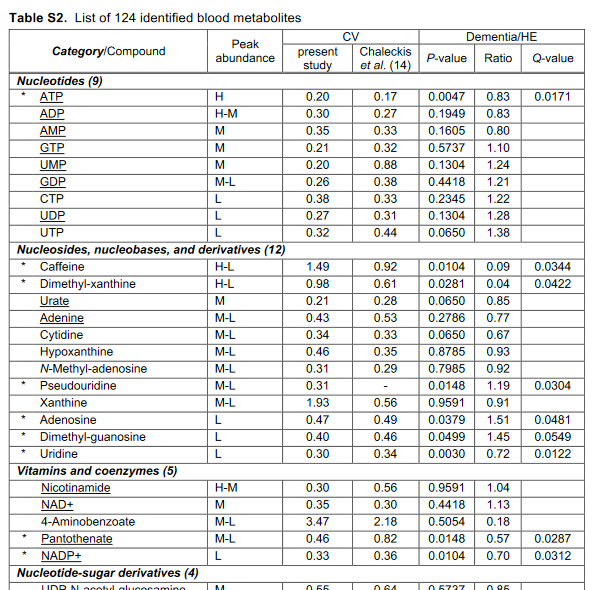
\includegraphics[width=0.8\textwidth]{img/multiple_hypothesis_correction/image-1715611965675.png}
    \caption*{The original Table S2 of \href{https://doi.org/10.1073/pnas.2022857118}{Teruya et al. (2021)}, which features incorrectly-calculated $q$ values.}
\end{figure}

\subsection*{Example 2: Lack of multiple hypothesis correction, inconsistency of $p$ values and $q$ values}

\href{https://doi.org/10.1096/fba.2020-00047}{Teruya et al. (2020)} report on performing metabolomics to determine if there are any metabolites that are present at different abundance in the urine of elderly individuals versus young individuals. They perform hypothesis testing on 99 metabolites, finding 55 out of 99 to be significantly different at unadjusted $p < 0.05$. Using an unadjusted $p$ value to determine significance instead of using multiple hypothesis correction in this case likely means that the majority of what the authors call significantly-different ``age-linked metabolites'' are actually false positives.

The authors do perform multiple hypothesis correciton with the Benjamini-Hochberg procedure, but appear not to use it for interpretation of their results. Instead, they state ``Q-values shown in Table S3 are consistent with p-values of 50 age-related compounds''.

However, the $q$ values shown in Table S3 do not increase monotonically with their corresponding $p$ values. There are some metabolites that depart wildly from the expected $q$ value, such as N-Acetyl-aspartate, with a $p$ value of 0.01675 and a $q$ value of 0.00045. It is not possible for any $q$ value to be less than its corresponding $p$ value.

\begin{figure}[h!tbp]
    \centering
    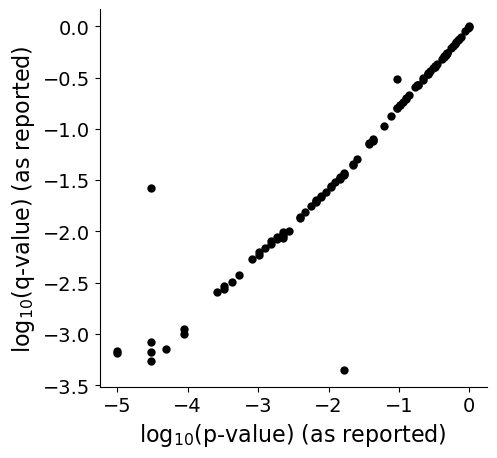
\includegraphics[width=0.8\textwidth]{img/multiple_hypothesis_correction/image-1715615096372.png}
    \caption*{A comparison of the $q$ values and $p$ values reported in Table S3 of \href{https://doi.org/10.1096/fba.2020-00047}{Teruya et al. (2020)}. Note that these $q$ values do not increase monotonically with their associated $p$ values, which should not be the case when using Benjamini-Hochberg correction.}
\end{figure}

\subsection*{Additional resources}

\begin{itemize}
    \setlength\itemsep{-0.5em}
    \item \href{https://doi.org/10.1378/chest.11-0523}{``Correction for multiple testing: is there a resolution?'' (2011)}
    \item \href{https://doi.org/10.1038/nbt1209-1135}{``How does multiple testing correction work?'' (2010)}
    \item \href{https://doi.org/10.4045/tidsskr.21.0357}{``Adjustment of p-values for multiple hypotheses'' (2021, available in Norwegian and English)}
\end{itemize}

\end{document}